As presented in section~\ref{sec:background}, Aligon's method~\cite{aligon2014similarity} can be used to compute the similarity between SQL queries. However, Aligon's method requires user to specify the weights of different parts of SQL queries that will be used in calculation of similarity. In this method, a SQL query is divided into three parts including \textit{projection}, \textit{group-by} and \textit{selection-join} (see Table~\ref{table:literaturereview} and Table~\ref{tab:features} for details). In this section, we explore the effect of choosing different weight for each query part in Aligon's method. 

\begin{figure*}[h!]
	\captionsetup[subfigure]{justification=centering}
    \centering
    \begin{subfigure}[b]{0.322\textwidth}%{0.48\textwidth}
        \centering
        %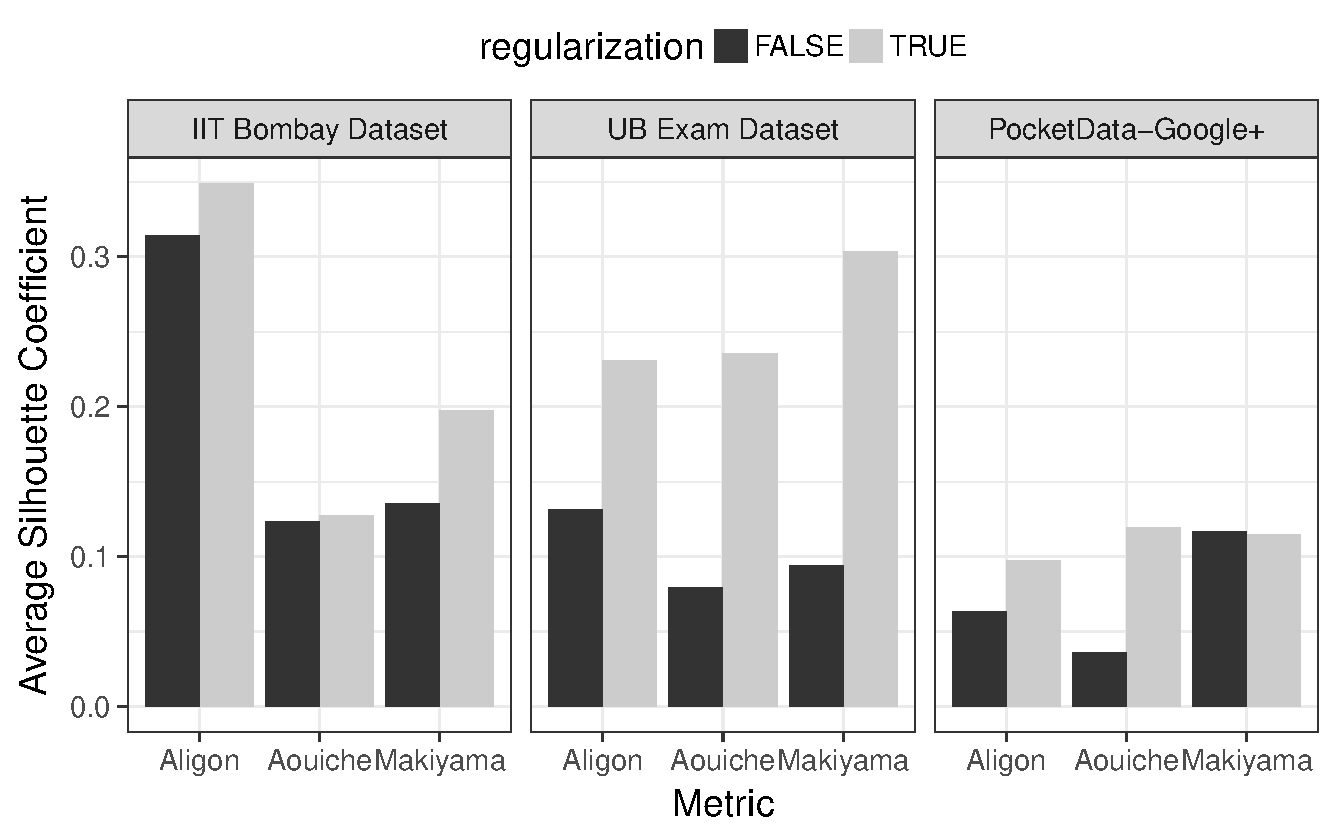
\includegraphics[width=\textwidth]{graphics/silhouette2}
        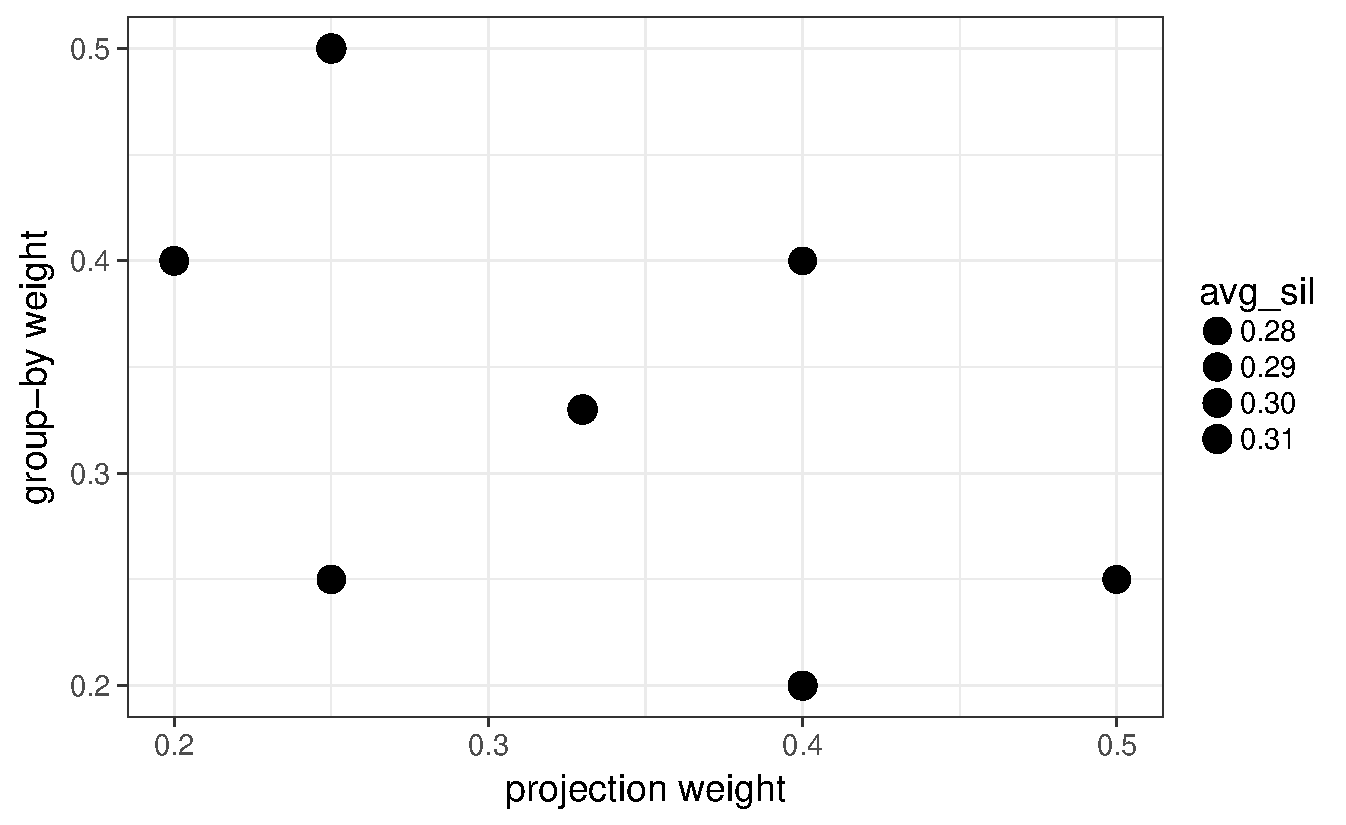
\includegraphics[width=\textwidth]{graphics/aligon_weight_bombay}
        \caption{IIT Bombay Dataset}
    \end{subfigure}%
    ~
    \begin{subfigure}[b]{0.322\textwidth}%{0.48\textwidth}
        \centering
        %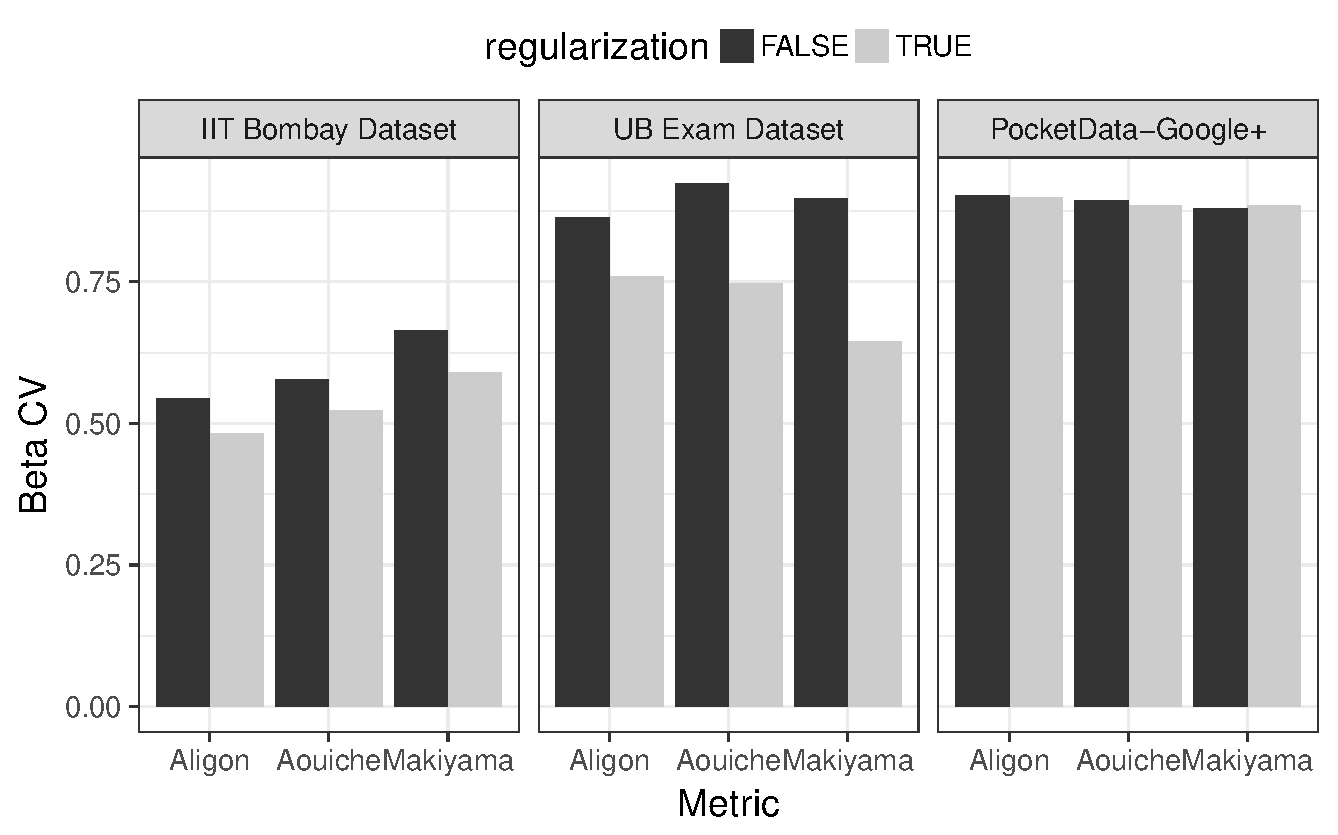
\includegraphics[width=\textwidth]{graphics/beta_cv2}
        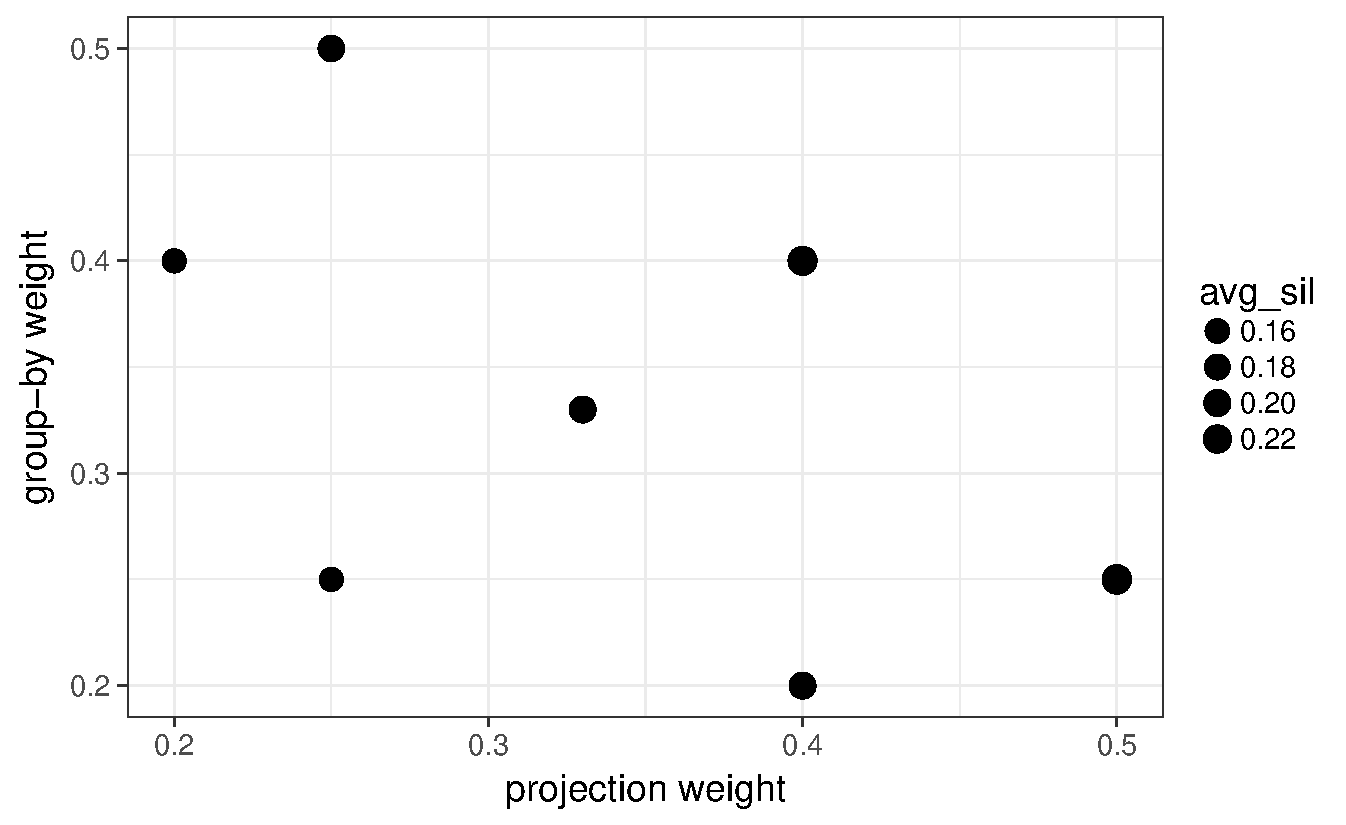
\includegraphics[width=\textwidth]{graphics/aligon_weight_ub}
        \caption{UB Exam Dataset}
    \end{subfigure}
    ~
    \begin{subfigure}[b]{0.322\textwidth}%{0.48\textwidth}
        \centering
        %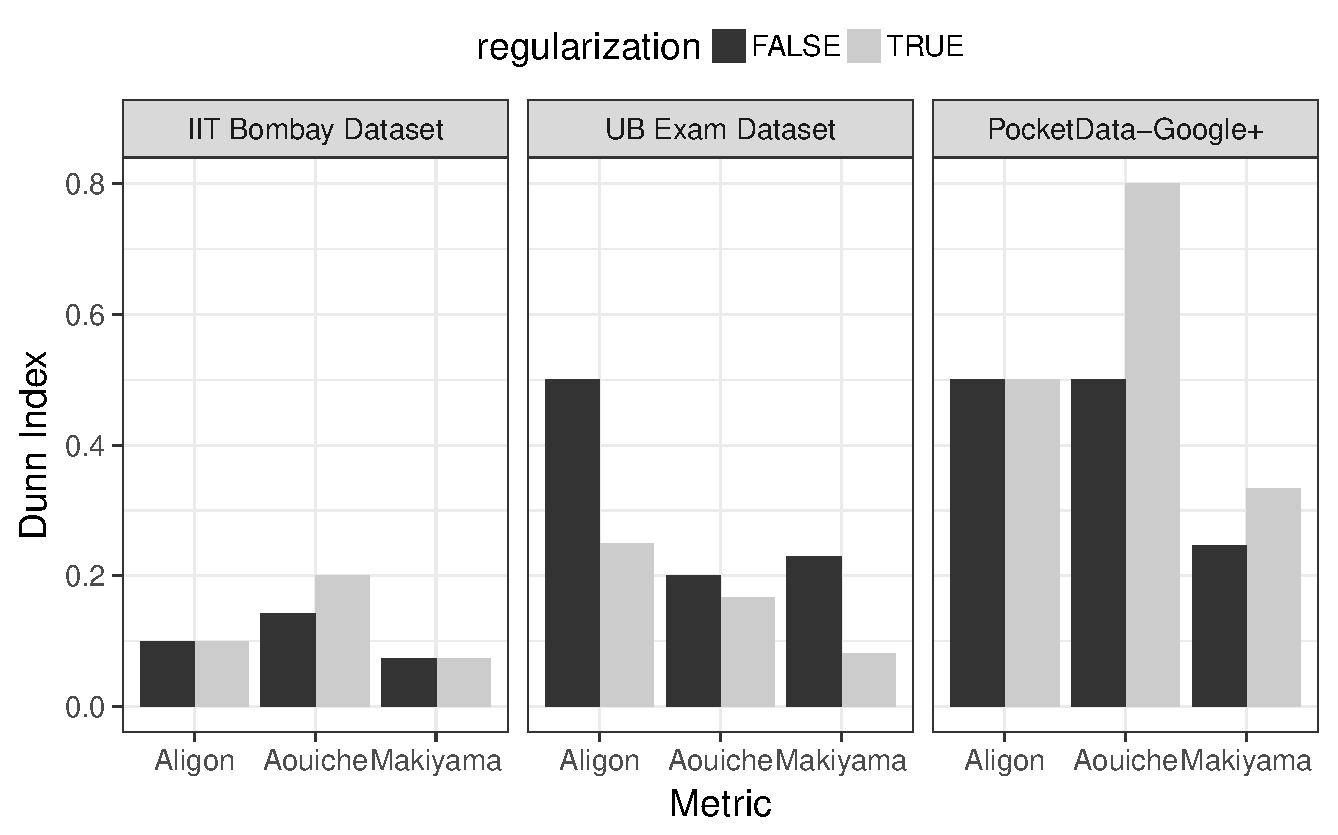
\includegraphics[width=\textwidth]{graphics/dunn2}
        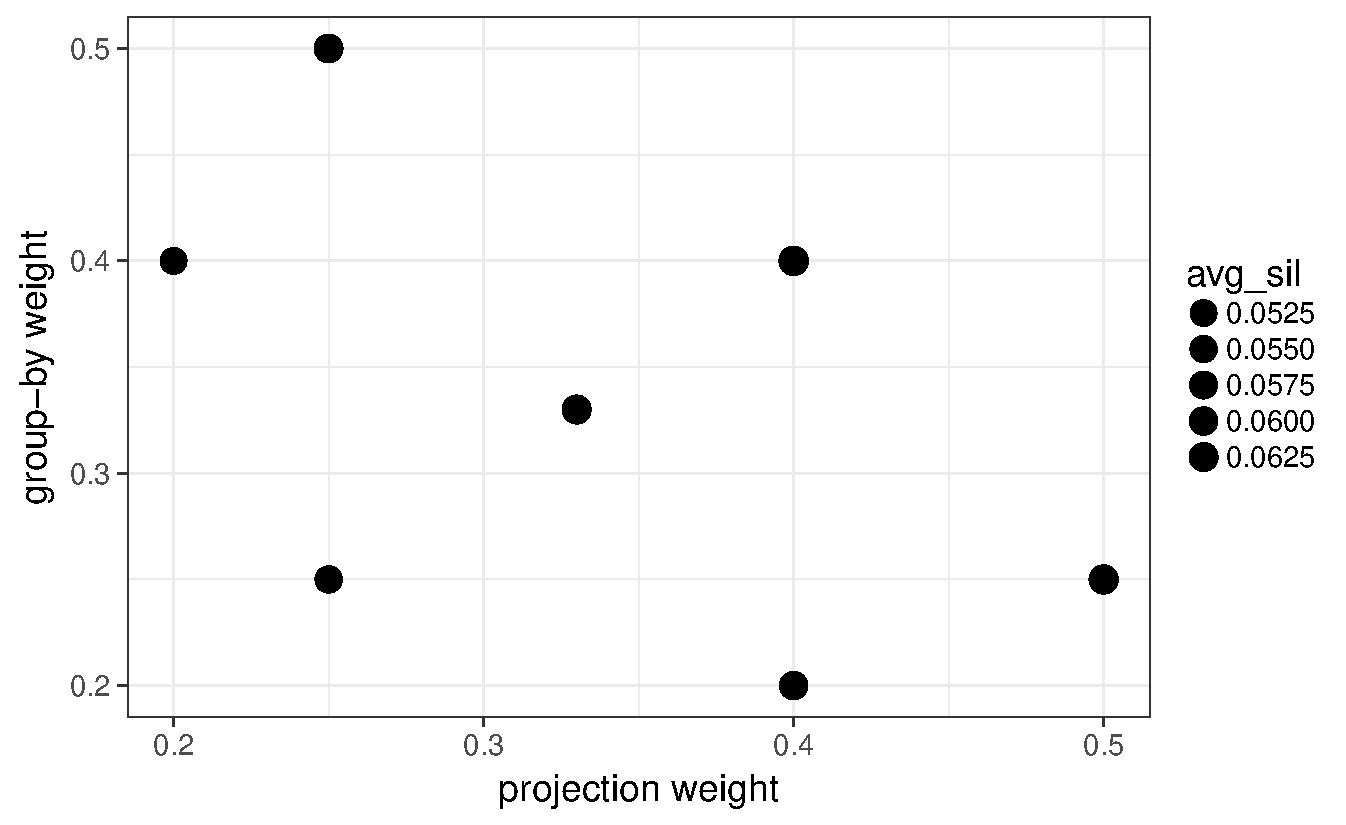
\includegraphics[width=\textwidth]{graphics/aligon_weight_googleplus}
        \caption{PocketData-Google+}
    \end{subfigure}
    \caption{Avergage Silhouette Coefficients with respect to different sets of weights in Aligon method}
    \label{fig:aligon_weight}
\end{figure*}

Let us denote a tuple $(w_{proj}, w_{select-join}, w_{groupby})$ as a set of weights for projection, selection-join and group-by respectively.Totally, we consider seven different combinations of weights including $(0.2, 0.4, 0.4)$, $(0.25, 0.25, 0.5)$, $(0.25, 0.5, 0.25)$, $(0.33, 0.33, 0.33)$, $(0.4, 0.2, 0.4)$, $(0.4, 0.4, 0.2)$ and $(0.5, 0.25, 0.25)$. 

Figure~\ref{fig:aligon_weight} presents the effect of different sets of weights in three datasets (see Section~\ref{subsec:data} for descriptions of these datasets). In this experiment, we use average Silhouette coefficient (see Section~\ref{subsec:validation} for further details) as a measure of quality for each combination of weights. In Aligon method, we have three weights, one for \textit{projection}, \textit{group-by} and \textit{selection-join} respectively, and the total of weights adding up to one. For this reason, we only present \textit{projection} weight and \textit{group-by} weight in Figure~\ref{fig:aligon_weight} as \textit{selection-join} weight can be computed by from \textit{projection} and \textit{group-by} weights. 

In Figure~\ref{fig:aligon_weight}, the size (area) of the point indicates the value of average Silhouette coefficient with respect to specific combination of weights. As can be seen in this figure, the values of average Silhouette coefficient change very little when adjusting the weights of projection and group-by. For this reason, in experiments shown in Section~\ref{sec:experiment}, we use equal weight for each query part, i.e. $(0.33, 0.33, 0.33)$, when applying Aligon's method to different datasets.

